\documentclass[landscape,pdftex]{jomislides}

\slidesmag{5} % escala, qto maior maiores ser�o as letras/figras/etc.

%\centerslidesfalse

\usepackage{algorithmic}

%
% Slides
% ======
%


\begin{document}

%\input{autorHeaders}

\title{Constraint Satisfaction Problems} 
\author{Fabr�cio Barth}
\institution{Insper}
\date{Outubro de 2022}

\SlideHeader{}
            {Intelig�ncia Artificial}
\SlideFooter{\theslidepartheading $\;$ --- $\;$ \theslideheading}
            {\theslide}

\vpagecolor[white]{white}


\subtitle{}

\maketitle

\begin{Slide}{\textbf{Problema das N rainhas}}
	
		Dado um tabuleiro $N \times N$, � poss�vel encontrar uma configura��o onde $N$ rainhas no tabuleiro n�o conseguem atacar nenhuma das outras rainhas no mesmo tabuleiro?
		
		\begin{center}
			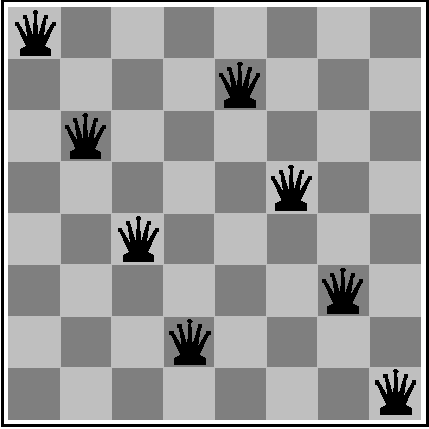
\includegraphics[width=.4\textwidth]{figuras/fig03-05.pdf}
		\end{center}
		
\end{Slide}


\begin{Slide}{Introdu��o}
	
	At� agora vimos diversos problemas de planejamento. Problemas onde o agente precisava sair de um estado e chegar em outro, ou seja, sequenciar um conjunto de a��es para alcan�ar um objetivo. 
	
	No entanto, existem outras classes de problemas onde o objetivo n�o est� em encontrar uma sequ�ncia de a��es, mas sim \textbf{encontrar um ou mais estados que satisfazem um conjunto de restri��es}.

\end{Slide}

\begin{Slide}{Algoritmo \textbf{Subida da Montanha}}
  \textbf{Id�ia}: escolher sempre um sucessor melhor

(``\textit{subir sempre}'').
 
\begin{algorithmic} 
\STATE \textbf{function} BSM-1(Estado $inicial$): Estado
\STATE Estado $atual \gets inicial$
\LOOP
    \STATE $prox \gets $ melhor sucessor de $atual$ (segundo $h$)
    \IF[sem sucessor melhor]{$h(prox) \geq h(atual)$}
       \STATE \textbf{return} $atual$
    \ENDIF
    \STATE $atual \gets prox$
\ENDLOOP
\end{algorithmic}
\end{Slide}

\begin{Slide}{\textbf{An�lise} do algoritmo BSM}
  \begin{itemize}
  \item N�o mant�m a �rvore (logo, n�o pode retornar o caminho que
    usou para chegar � meta).

  \item Completo:  \textbf{n�o} (problema de \emph{m�ximos locais})
  \item �timo:  n�o se aplica
  \item Tempo:  \textbf{?}
  \item Espa�o:  \textbf{nada}!
  \end{itemize}
\end{Slide}


\begin{Slide}{Algoritmo \textbf{Subida da Montanha Estoc�stico}}
{\footnotesize
\begin{algorithmic} 
\STATE \textbf{function} BSM-2(Estado $inicial$): Estado
\STATE Estado $atual \gets inicial$
\LOOP
    \STATE $prox \gets $ melhor sucessor de $atual$ (segundo $h$)
    \IF[sem sucessor melhor]{$h(prox) \geq h(atual)$}
       \IF{$atual$.\textbf{�Meta}()}
          \STATE \textbf{return} $atual$
       \ELSE
          \STATE $atual \gets$ estado gerado aleat�riamente
       \ENDIF
    \ELSE
       \STATE $atual \gets prox$
    \ENDIF
\ENDLOOP
\end{algorithmic}
}
\end{Slide}


\begin{Slide}{\textbf{An�lise} do algoritmo BSM Estoc�stico}
  \begin{itemize}
  \item Completo:  \textbf{sim} (se a gera��o de estados
    aleat�rios tiver uma distribui��o uniforme)
  \item �timo:  n�o se aplica
  \item Tempo:  \textbf{?}
  \item Espa�o:  \textbf{nada}!
  \end{itemize}
\end{Slide}


\begin{Slide}{Material de \textbf{consulta}}
  \begin{itemize}
  \item Cap�tulo 5 do livro do Russell \& Norvig
  \end{itemize}
\end{Slide}


\end{document}

